\documentclass[letterpaper,12pt]{report}
%
%--------------------   start of the 'preamble'
%
\usepackage{graphicx,amssymb,amstext,amsmath,url}
%
%%    homebrew commands -- to save typing
\newcommand\etc{\textsl{etc}}
\newcommand\eg{\textsl{eg.}\ }
\newcommand\etal{\textsl{et al.}}
\newcommand\Quote[1]{\lq\textsl{#1}\rq}
\newcommand\fr[2]{{\textstyle\frac{#1}{#2}}}
\newcommand\miktex{\textsl{MikTeX}}
\newcommand\comp{\textsl{The Companion}}
\newcommand\nss{\textsl{Not so Short}}
%
%---------------------   end of the 'preamble'
%

\begin{document}
%-----------------------------------------------------------
\title{Multi-Agent Lab \\
{\large \textbf{CS 470 Lab 3}}}
\author{Duane Johnson, Michael Ries and Jon Brandenburg}
\maketitle
%-----------------------------------------------------------
\begin{abstract}
This lab is all about coordination and higher-level algorithms that can be used to control agents.
Specifically this lab asks the students to implement a decoy tactic in which the enemy tanks are kept
busy shooting at a decoy while a second tank aims and shoots the enemy tanks.  In addition to the
added complexity of the decoy-sniper coordination the students are also required to use search paths to
find their way through a maze and get to a location.
\end{abstract}
%-----------------------------------------------------------
\tableofcontents
%-----------------------------------------------------------
\chapter{Lab Context}\label{chap:context}
\section{Summary}
The authors each developed and ran the software below on laptops.  The laptops were unix-based systems; however, these results should be easily duplicated on a Windows machine.

\section{Hardware}
\begin{itemize}
    \item Macbook Pro (32 bit) / 2.4 GHz Intel Core 2 Duo / 2 GB RAM
    \item Lenovo T400 (32 bit) / 2.2 GHz Intel Core 2 Duo / 2 GB RAM
    \item HP Pavilion (64 bit) / 2.5 GHz Intel Core 2 Duo / 4 GB RAM
\end{itemize}

\section{Software}
\begin{itemize}
    \item Mac OS X 10.5
    \item Ubuntu 9.04
    \item bzFlag 2.0.7 with patched bzrobots client\footnote{Supplied by CS470 in \textsl{Install Instructions}}
    \item Ruby Interpreter, version 1.8.7 (or 1.9.1)
    \item EventMachine Library\footnote{\url{http://rubyeventmachine.com/}} for Ruby
    \item PDF-Writer Library\footnote{\url{http://ruby-pdf.rubyforge.org/pdf-writer/}} for Ruby
    \item Rake Library\footnote{\url{http://rake.rubyforge.org/}} for Ruby Unit Tests
    \item NArray and NMatrix \footnote{\url{http://narray.rubyforge.org/}} for Ruby
\end{itemize}

\chapter{Experiences and Time Spent}\label{chap:exp}
\section{Duane's Summary}
My assignment for this project was primarily to implement the Kalman filter and to show its output in PDF form for the report.  It was actually quite fun to turn the Kalman math into code using Ruby's NArray gem.  Because Ruby supports operator overloading, the matrix math was nearly as easy to code up as any algebraic equation.  We had to tweak the timing variable a bit so that our $t+1$ matrices properly represented the ``next iteration'' of the cycle.
\par
The ``screenshots'' in this report were produced using PDF output.  Part of my contribution was to generate the non-Kalman and Kalman paths for this output.
\par
I spent about 11 hours on this project, divided as follows:
\begin{itemize}
    \item 5 hours implementing the Kalman Filter in Ruby
    \item 3 hours merging code with Michael and passing off with another team in the lab
    \item 2 hours writing new PDF output with kalman paths
    \item 1 hour taking screenshots of the kalman paths
\end{itemize}

\section{Michael's Summary}
This week I started off trying to debug why our agents from the last lab kept getting stuck after capturing the enemy flag. I spent part of Sunday and Monday night tracing the problem through our code
and finally found it late Monday night.  The problem turned out to be related to caching the search path
and not re-calculating it when we had purposely cleared the cached search path.
\par
Later in the week I got to work on fixing up our PD controller to be more accurate for following paths.  This task - like the task above - was not directly related to the passof for this lab, but was a necessary step to making sure our team would be ready for the final lab.
\par
Finally towards the latter part of the week I spent my time on the aiming/shooting code.  I investigated 6 different methods of calculating the intersection of vectors.  I tried several different methods of treating the vectors as parametric equations as well as solving the problem as a system of linear equations and even some trigonometry.  In the end the a simple iterative approach proved to be the fastest while maintaining the same level of accuracy as the others.
\par
At the end of the week I had spent a total of 28 hours in the following areas:
\begin{itemize}
    \item 4 hours fixing the bug from last lab.
    \item 4 hours working on the PD controller to get better path following.
    \item 6 hours researching vector intersection methods
    \item 8 hours implementing several aim/shoot ideas
    \item 4 hours meeting with the team to passoff the lab
    \item 2 hours compiling report materials
\end{itemize}

\section{Jon's Summary}
I spent roughly five hours writing and testing all of the clay pigeons.
\chapter{Details}\label{chap:details}
\section{Path Following and Potential Fields}
While developing our search algorithms in the last lab we realized that doing full $A*$ searching was not going to be possible in ruby if our discretization was too granular. To alleviate this problem Duane Johnson developed a small library written in C which acted as a module to the rest of our code.  We also simplified the representation of the discretized map for the algorithm to search through.  With these changes we were able to search through maps of 80x80 in approximately 1/10 of a second.  This was fast enough and granular enough for the purpose of finding our way through a maze and deploying a decoy-sniper tactic.
\par
When it came time to follow the solution path returned by Duane's $A*$ module the immediate thought was to use potential fields along the length of the path.  The potential fields code developed in the first lab already had a PD controller which would suggest velocity and angular velocity based on the current position and angle of the tank.  As the lab progressed we optimized this algorithm to actually look as far ahead as the line segments are parallel so that when driving in a straight line we don't spend much time re-evaluating the path.  We also periodically re-evaluate the search solution which will be important in the future when we are trying to avoid enemy tanks and our world becomes more dynamic.
\par
In addition to the path following optimizations we also 'tuned' the relative strength of the fields and their radii so that as we approach the next Potential Field the system will move it to the next location before our arrival.  This helped to avoid uneccesary 'braking' and turning.

\section{Tests with Another Group}
\subsection{Our Tests}
We ran the tests for our implementation on the astar.bzw map from the lab website. Our tests went well with the exception of the return trip to our base after capturing the flag.  This is the one odd behavior for which no solution has yet been found.
\par
\begin{figure}\label{fig:stuck}
\begin{center}
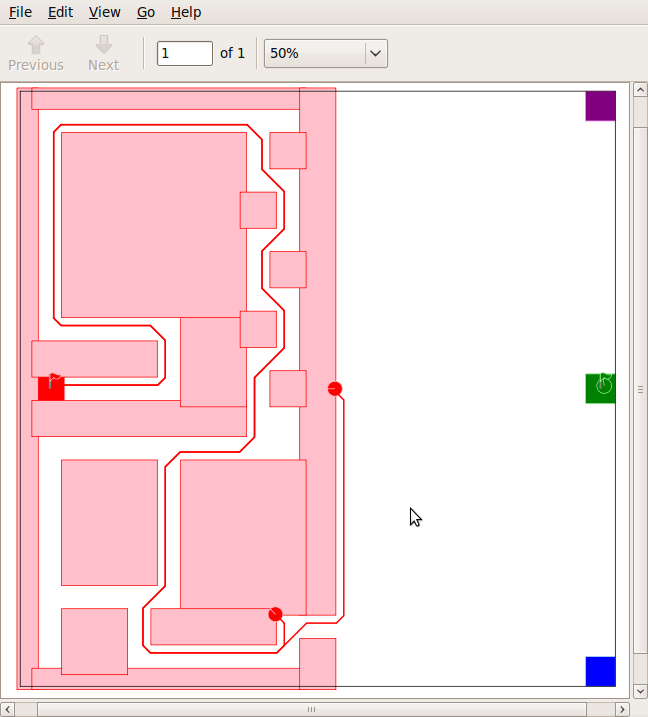
\includegraphics[width=\textwidth]{07re-evaluate-path.png}
\caption{Getting stuck at the wall on the way home. Re-evaluated path show}
\end{center}
\end{figure}
After we capture the flag the sniper agent is given the task to search for a path home, but always gets stuck against a wall and will remain stuck until the search path is re-evaluated. Once the path is re-evaluated we returned to home base successfully.  This is a problem we will need to fix in subsequent labs, but which did not stop us from passing this lab.

\subsection{Michael Hansen and Daniel Nelson}
We ran our tests with another group from class which consisted of:
\begin{itemize}
    \item{Michael Hansen}
    \item{Daniel Nelson}
\end{itemize}
What was interesting about watching the other team pass off was that they had a few problems in their implementation, but they were in no way related to the problems we encountered.  The main problem the other team had was that the decoy would get killed as it went into its decoy mode.  They had to change the timing of their agents to avoid this, but in the end they successfully completed the challenge.
%-----------------------------------------------------------
% \addcontentsline{toc}{chapter}{\numberline{}Bibliography}
%\include{biblio}
%-----------------------------------------------------------
\appendix
\chapter{Ruby Code}\label{app:code}
Listed below is the partial source of our Ruby search implementation. A complete listing of our project's code was included in the first lab report.  Since much of our code is the same as Lab 1, we have not duplicated it here.
\par

\section{search.rb}
\begin{verbatim}
bzrequire 'lib/agent/basic'
bzrequire 'lib/collection/stack'
bzrequire 'lib/collection/queue'
bzrequire 'lib/collection/priority_queue'
require 'set'

module BraveZealot
  module Agent
    class Search < Basic
      def to_gnuplot
        str = @hq.map.to_gnuplot
        last = nil
        s = @n
        if $options.debug then
          get_log.each do |n|
            if !last.nil?  then
              str += "set arrow from #{last.center.x}, #{last.center.y} " +
                     "to #{n.center.x}, #{n.center.y} nohead lt 5\n"
              str += "plot '-' with lines\n"
              str += " 0 0 0 0\n"
              str += "e\n"
              str += "pause 0.005000\n"
            end
            last = n
          end
        end
        puts "Flag at #{@hq.map.goal.to_coord.inspect} -> Our solution is " +
             "#{s.to_coord.inspect} (#{s.actual_cost} -> " +
             "#{s.predecessors.size + 1}) Nodes popped: #{get_log.size}"
        last = s
        list = s.predecessors
        s.predecessors.each do |n|
          if !last.nil?  then
            str += "set arrow from #{last.center.x}, #{last.center.y} to " +
                   "#{n.center.x}, #{n.center.y} nohead lt 1\n"
            str += "plot '-' with lines\n"
            str += " 0 0 0 0\n"
            str += "e\n"
            str += "pause 0.005000\n"
          end
          last = n
        end
        str
      end

      def save_gnuplot
        f = File.new($options.gnuplot_file,'w')
        f.write(to_gnuplot)
        f.close
        puts "Finished!"
        $stdout.flush
      end

      def log(n)
        @log ||= []
        @log << n
      end

      def get_log
        @log ||= []
      end
    end

    class UninformedSearch < Search

      protected

      def search(init, fringe, limit = 0)
        limited = false
        closed = Set.new
        fringe = fringe.insert(init)
        loop do
          # puts closed.size
          # puts
          if fringe.empty?
            puts "Done search: #{limit}"
            return (limited ? :limited : false)
          end
          node = fringe.remove
          log(node)
          if node.goal?
            puts "Done search: found"
            @n = node
            return node
          end
          if !closed.include?(node)
            closed.add(node)
            size = node.predecessors.size
            if size < limit
              node.succ.each do |n|
                n2 = n.clone
                n2.predecessors = ( node.predecessors.clone ) << node
                fringe.insert(n2)
              end
            else
              limited = true
            end
            # fringe.insert_all(node.succ)
          end
        end
      end
    end

    class DepthFirstSearch < UninformedSearch
      def start
        init = @hq.map.chunk_at_point(@tank.x, @tank.y)
        fringe = Collection::Stack.new
        search(init, fringe)
        save_gnuplot
      end
    end

    class DepthLimitedSearch < UninformedSearch
      def start
        init = @hq.map.chunk_at_point(@tank.x, @tank.y)
        iter_search(init)
        save_gnuplot
      end

      def iter_search(init)
        i = 1
        while (search([init], i)) == :limited
          puts "Iter depth: #{i}"
          i += 1
        end
      end

      def search(list, limit)
        (return :limited) if list.size > limit
        me = list.first
        return me if me.goal?
        puts "I am chunk #{me.x}, #{me.y}"
        log(me)
        result = false
        me.succ.each do |s|
          unless list.include?(s)
            puts ("  " * (list.size - 1)) + "successor #{s.x}, #{s.y}"
            s.predecessors = list.clone
            result = search([s] + list, limit)
            # p result.class
            # If it's a goal node, return right away
            return (@n = result) if result.is_a?(Chunk)
          end
        end
        # The last result will either be 'false' or :limited, and
        # we should return it in either case
        return result
      end

    end

    class BreadthFirstSearch < UninformedSearch
      def start
        init = @hq.map.chunk_at_point(@tank.x, @tank.y)
        fringe = Collection::Queue.new
        search(init, fringe)
        save_gnuplot
      end
    end

    class InformedSearch < Search
      def start
        init = @hq.map.chunk_at_point(@tank.x, @tank.y)
        fringe = Collection::PriorityQueue.new
        @n = search(init, fringe)
        save_gnuplot
      end

      def search(init, fringe)
        closed = Set.new
        fringe.insert(init)
        loop do
          return false if fringe.empty?
          node = fringe.remove
          return node if node.goal?
          if !closed.include?(node)
            log(node)
            closed.add(node)
            # This is where informed searches are different we must evaluate
            # a priority before pushing onto the priority queue
            node.succ.each do |n|
              n2 = n.clone
              n2.g = node.g + (node.center.vector_to(n.center).length)
              n2.predecessors = ( node.predecessors.clone ) << node
              fringe.insert(n2)
            end
          end
        end
      end
    end

    class GreedyInformedSearch < InformedSearch
      def search(init, fringe)
        closed = Set.new
        fringe.insert(init)
        loop do
          return false if fringe.empty?
          node = fringe.remove
          return node if node.goal?
          if !closed.include?(node)
            log(node)
            closed.add(node)
            # This is where informed searches are different we must evaluate
            # a priority before pushing onto the priority queue
            node.succ.each do |n|
              n2 = n.clone
              n2.predecessors = ( node.predecessors.clone ) << node
              fringe.insert(n2)
            end
          end
        end
      end
    end
  end
end
\end{verbatim}


\section{stack.rb}
\begin{verbatim}
bzrequire 'lib/collection/base'

module Collection
  class Stack < Base
    def insert(e)
      @data.push(e)
      self
    end
    def remove
      @data.pop
    end
  end
end
\end{verbatim}

\section{queue.rb}
\begin{verbatim}
bzrequire 'lib/collection/base'

module Collection
  class Queue < Base
    def insert(e)
      @data << e
      self
    end
    def remove
      @data.shift
    end
  end
end
\end{verbatim}

\section{priority\textunderscore queue.rb}
\begin{verbatim}
bzrequire 'lib/collection/containers/priority_queue'

module Collection
  class PriorityQueue < Base
    def initialize
      @pq = Containers::PriorityQueue.new()
    end

    def insert(e)
      # We can just make sure that each Chunk can return a
      # priority for us.  We negate the priority so that we
      # get a priority that returns the 'smallest' priority
      # first instead of the 'biggest' priority first.
      @pq.push(e, -1*e.priority)
    end

    def remove
      @pq.pop
    end

    def size
      @pq.size
    end

    def empty?
      @pq.empty?
    end
  end
end
\end{verbatim}
%\include{app1}
%\include{app2}
%\include{app5}
%\include{app3}
%-----------------------------------------------------------
\end{document}
